\documentclass[11pt,a4paper,english]{article}
\usepackage[utf8]{inputenc}
\usepackage[T1]{fontenc}
%\usepackage{babel}
%\usepackage{fancyhdr}
\usepackage{amsfonts,amsmath,amssymb,pifont,enumerate,graphicx,textcomp,varioref,algpseudocode,listings}
\usepackage[margin=1in,footskip=0.25in]{geometry}

\title{MEK3220 - Formulae sheet}
\author{Krister Stræte Karlsen}
\tolerance = 5000 
\hbadness = \tolerance 
\pretolerance = 2000 

\usepackage{color}
\usepackage{listings}
\usepackage{setspace}
\usepackage{framed}

\definecolor{Code}{rgb}{0,0,0}
\definecolor{Decorators}{rgb}{0.5,0.5,0.5}
\definecolor{Numbers}{rgb}{0.5,0,0}
\definecolor{MatchingBrackets}{rgb}{0.25,0.5,0.5}
\definecolor{Keywords}{rgb}{0,0,1}
\definecolor{self}{rgb}{0,0,0}
\definecolor{Strings}{rgb}{0,0.63,0}
\definecolor{Comments}{rgb}{0,0.63,1}
\definecolor{Backquotes}{rgb}{0,0,0}
\definecolor{Classname}{rgb}{0,0,0}
\definecolor{FunctionName}{rgb}{0,0,0}
\definecolor{Operators}{rgb}{0,0,0}
\definecolor{Background}{rgb}{0.98,0.98,0.98}

\lstnewenvironment{python}[1][]{
\lstset{
numbers=left,
numberstyle=\footnotesize,
numbersep=1em,
xleftmargin=1em,
framextopmargin=2em,
framexbottommargin=2em,
showspaces=false,
showtabs=false,
showstringspaces=false,
frame=l,
tabsize=4,
% Basic
basicstyle=\ttfamily\small\setstretch{1},
backgroundcolor=\color{Background},
language=Python,
% Comments
commentstyle=\color{Comments}\slshape,
% Strings
stringstyle=\color{Strings},
morecomment=[s][\color{Strings}]{"""}{"""},
morecomment=[s][\color{Strings}]{'''}{'''},
% keywords
morekeywords={import,from,class,def,for,while,if,is,in,elif,else,not,and,or,print,break,continue,return,True,False,None,access,as,,del,except,exec,finally,global,import,lambda,pass,print,raise,try,assert},
keywordstyle={\color{Keywords}\bfseries},
% additional keywords
morekeywords={[2]@invariant},
keywordstyle={[2]\color{Decorators}\slshape},
emph={self},
emphstyle={\color{self}\slshape},
%
}}{}

\lstset{keywordstyle=\color{kewwords},backgroundcolor=\color{mygray},basicstyle=\footnotesize\ttfamily,breaklines=true,commentstyle=\color{mygray},language=Python,firstline=1,lastline=53,frame=single,numbers=left,numberstyle=\tiny\color{mygray}}


\begin{document}
\maketitle

{\scshape The displacement gradient} \\

\begin{align*}
\nabla \mathbf{u} = 
\begin{pmatrix}	    \frac{\partial u_x}{ \partial x} & \frac{\partial u_x}{ \partial y} & \frac{\partial u_x}{ \partial z}      \\
                		\frac{\partial u_y}{ \partial x} & \frac{\partial u_y}{ \partial y} & \frac{\partial u_y}{ \partial z}     \\
               	 	\frac{\partial u_z}{ \partial x} & \frac{\partial u_z}{ \partial y} &\frac{\partial u_z}{ \partial z}     
\end{pmatrix}
\end{align*}
\\[1ex] 
Comment: If $ \nabla \mathbf{u} =  ( \nabla \mathbf{u})^T  $ we have that $\nabla \mathbf{u} = \epsilon $, the \emph{strain tensor}.
\\[2ex] 

{\scshape Strain tensor} \\
\begin{align*}
\epsilon = \frac{1}{2}( (\nabla \mathbf{u} )^T + \nabla \mathbf{u}  ) 
\end{align*}
\\[2ex] 

{\scshape Cauchy's equilibrium equation} \\
\begin{align*}
\mathbf{f_v} + \nabla \cdot \sigma^T = 0
\end{align*}
\\[2ex]

{\scshape Hooke's law} \\
\begin{align*}
\{\sigma \} = \lambda (\nabla \cdot \mathbf{u}) I + \mu \epsilon
\end{align*}
or 
\begin{align*}
\sigma_{xx} = (2\mu + \lambda) \epsilon_{xx} + \lambda (\epsilon_{yy} + \epsilon_{zz}), \quad \sigma_{yz} = \sigma_{zy} = 2 \mu \epsilon_{yz} \\
\sigma_{yy} = (2\mu + \lambda) \epsilon_{yy} + \lambda (\epsilon_{xx} + \epsilon_{zz}), \quad \sigma_{xz} = \sigma_{zx} = 2 \mu \epsilon_{xz}  \\
\sigma_{zz} = (2\mu + \lambda) \epsilon_{zz} + \lambda (\epsilon_{yy} + \epsilon_{zz}), \quad \sigma_{xy} = \sigma_{yx} = 2 \mu \epsilon_{xy} 
\end{align*}
\\[2ex]

{\scshape Inverted Hooke's law} \\
\\[2ex]

{\scshape Navier's equation for elastic media in motion} \\
\begin{align*}
\frac{\partial^2 \mathbf{u}}{\partial t^2} = \mu \nabla^2 \mathbf{u} + (\lambda + \mu) \nabla \nabla \cdot \mathbf{u} + \mathbf{f_v}
\end{align*}
\\[1ex] 
Comment: For mechanical equilibrium set LHS. equal to zero. 
\\[2ex]

{\scshape Lamè coefficients} \\
\\[2ex]

{\scshape Beam equations} \\

\emph{Euler-Bernoulli} and some additional important relations

\begin{figure}[h!]
\centering
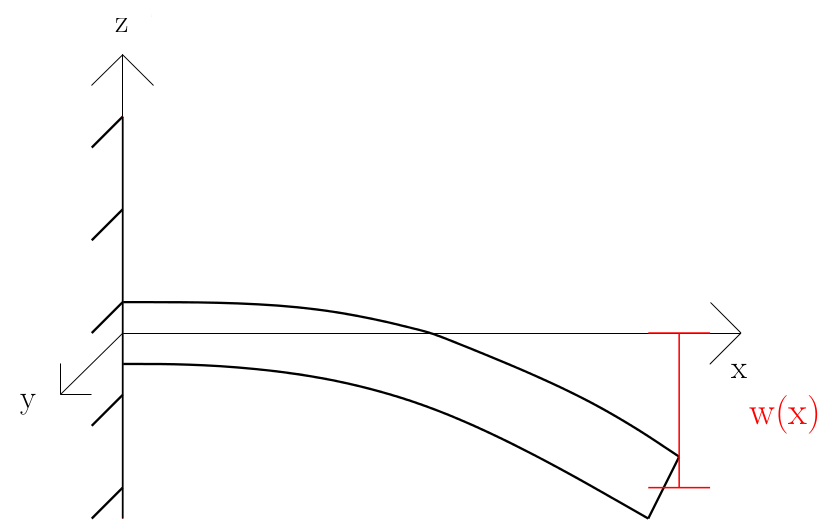
\includegraphics[scale=0.15]{figures/beam.png}
\end{figure}


\begin{align*}
\frac{d^2 w(x)}{dx^2} = - \frac{M_y (x)}{EI}, \quad \frac{dM_y(x)}{dx} = F_z, \quad \frac{dF_z}{dx} = - F_{ext}^{(z)} 
\end{align*}
\\[2ex]

{\scshape Equation of continuity} \\
\begin{align*}
\frac{\partial \rho}{\partial t} + \nabla \cdot  \rho \mathbf{v} = 0
\end{align*}
\\[2ex]

{\scshape Navier-Stokes} \\
\begin{align*}
\frac{d \mathbf{v}}{dt} + (\mathbf{v} \cdot \nabla)\mathbf{v} = \mathbf{g} - \frac{1}{\rho} \nabla p + \nu \nabla^2 \mathbf{v}, \quad \nabla \cdot \mathbf{v} = 0  
\end{align*}
\\[2ex]

{\scshape Viscous shear stress} \\
\\[2ex]

{\scshape Energy equations} \\

Kinetic energy(per volume) for fluid:
\begin{align*}
E_k = \frac{1}{2} \rho \mathbf{v}^2 = \frac{1}{2} \rho (u^2 + v^2 + w^2) 
\end{align*}

Work done by wall(at $y=h$ with length: $L$) from shear stress($\sigma_{xy}$) on fluid:
\begin{align*}
W = U(h) L \sigma_{xy}(h)
\end{align*}

[add figure]



\end{document}



\grid
